\documentclass[12pt,(landscape,a4paper),(portrait,a4paper)]{article}
\usepackage{lmodern}
\usepackage{amssymb,amsmath}
\usepackage{ifxetex,ifluatex}
\usepackage{fixltx2e} % provides \textsubscript
\ifnum 0\ifxetex 1\fi\ifluatex 1\fi=0 % if pdftex
  \usepackage[T1]{fontenc}
  \usepackage[utf8]{inputenc}
\else % if luatex or xelatex
  \ifxetex
    \usepackage{mathspec}
  \else
    \usepackage{fontspec}
  \fi
  \defaultfontfeatures{Ligatures=TeX,Scale=MatchLowercase}
\fi
% use upquote if available, for straight quotes in verbatim environments
\IfFileExists{upquote.sty}{\usepackage{upquote}}{}
% use microtype if available
\IfFileExists{microtype.sty}{%
\usepackage{microtype}
\UseMicrotypeSet[protrusion]{basicmath} % disable protrusion for tt fonts
}{}
\usepackage[margin=1in]{geometry}
\usepackage{hyperref}
\hypersetup{unicode=true,
            pdftitle={计量经济学Eviews实验指导书},
            pdfauthor={胡华平},
            pdfborder={0 0 0},
            breaklinks=true}
\urlstyle{same}  % don't use monospace font for urls
\usepackage{longtable,booktabs}
\usepackage{graphicx,grffile}
\makeatletter
\def\maxwidth{\ifdim\Gin@nat@width>\linewidth\linewidth\else\Gin@nat@width\fi}
\def\maxheight{\ifdim\Gin@nat@height>\textheight\textheight\else\Gin@nat@height\fi}
\makeatother
% Scale images if necessary, so that they will not overflow the page
% margins by default, and it is still possible to overwrite the defaults
% using explicit options in \includegraphics[width, height, ...]{}
\setkeys{Gin}{width=\maxwidth,height=\maxheight,keepaspectratio}
\IfFileExists{parskip.sty}{%
\usepackage{parskip}
}{% else
\setlength{\parindent}{0pt}
\setlength{\parskip}{6pt plus 2pt minus 1pt}
}
\setlength{\emergencystretch}{3em}  % prevent overfull lines
\providecommand{\tightlist}{%
  \setlength{\itemsep}{0pt}\setlength{\parskip}{0pt}}
\setcounter{secnumdepth}{5}
% Redefines (sub)paragraphs to behave more like sections
\ifx\paragraph\undefined\else
\let\oldparagraph\paragraph
\renewcommand{\paragraph}[1]{\oldparagraph{#1}\mbox{}}
\fi
\ifx\subparagraph\undefined\else
\let\oldsubparagraph\subparagraph
\renewcommand{\subparagraph}[1]{\oldsubparagraph{#1}\mbox{}}
\fi

%%% Use protect on footnotes to avoid problems with footnotes in titles
\let\rmarkdownfootnote\footnote%
\def\footnote{\protect\rmarkdownfootnote}

%%% Change title format to be more compact
\usepackage{titling}

% Create subtitle command for use in maketitle
\newcommand{\subtitle}[1]{
  \posttitle{
    \begin{center}\large#1\end{center}
    }
}

\setlength{\droptitle}{-2em}
  \title{计量经济学Eviews实验指导书}
  \pretitle{\vspace{\droptitle}\centering\huge}
  \posttitle{\par}
\subtitle{Lab 3 模型函数形式与模型选择}
  \author{胡华平}
  \preauthor{\centering\large\emph}
  \postauthor{\par}
  \predate{\centering\large\emph}
  \postdate{\par}
  \date{2018/3/22}

\usepackage{xeCJK}
\setCJKmainfont{楷体}  % 字体可以更换
\setmainfont{Georgia} % 設定英文字型
\setromanfont{Georgia} % 字型
\setmonofont{Courier New}

%设置版式 垂直或水平
% You know, for landscape
\usepackage{lscape}
\usepackage{pdfpages}


% Make new page before each section
\let\stdsection\section
\renewcommand\section{\newpage\stdsection}

% pandoc does not parse latex env - https://groups.google.com/forum/?fromgroups=#!topic/pandoc-discuss/oZETB5Ii1Cw
\newcommand{\blandscape}{\begin{landscape}}
\newcommand{\elandscape}{\end{landscape}}

\begin{document}
\maketitle

\renewcommand{\figurename}{图}
\renewcommand{\contentsname}{目录}
\renewcommand{\tablename}{表}

%% maxwidth is the original width if it's less than linewidth
%% otherwise use linewidth (to make sure the graphics do not exceed the margin)
\makeatletter
\def\maxwidth{ %
  \ifdim\Gin@nat@width>\linewidth
    \linewidth
  \else
    \Gin@nat@width
  \fi
}
\makeatother

{
\setcounter{tocdepth}{3}
\tableofcontents
}
\section{实验目的及要求}

\begin{itemize}
\tightlist
\item
  \textbf{目的}:掌握几种模型函数形式的特征,理解函数形式选择的原理。
\item
  \textbf{要求}:在老师指导下能用Eviews软件进行各种形式模型的变换与处理,包括普通线性模型、过原点模型、标准化处理模型、双对数模型、半对数模型、倒数模型,得到正确的分析结果;能运用合适的计算公式,得到正确的斜率和弹性计算值。
\end{itemize}

\section{实验原理}

\begin{itemize}
\tightlist
\item
  无论是一元线性回归还是多元线性回归,模型正确设置的一个重要前提就是能够正确地选择合适的函数形式,或者需要对变量进行变换处理(标准化、取对数等)。同样的实证案例,使用普通线性模型、过原点模型、标准化处理模型、双对数模型、半对数模型、倒数模型需要视案例具体情形而定,还需要结合经济学理论,通过多次尝试方才能够找到相对满意的具体模型形式。
\item
  此外,斜率和弹性,都是具有数学和经济学含义的重要概念,不同函数形式下实现对二者的正确计算,是得出有价值的模型估计结论的重要途径。
\end{itemize}

\section{实验内容}

\subsection{实验方案设计}

\begin{itemize}
\item
  进行不同模型形式的Eviews操作,包括过原点模型、标准化处理模型、双对数模型、半对数模型、倒数模型。
\item
  学会计算不同模型形式下Y对X的斜率和弹性公式。
\end{itemize}

\begin{longtable}[]{@{}llll@{}}
\caption{模型函数形式及计算 \label{modelslc}}\tabularnewline
\toprule
\begin{minipage}[b]{0.18\columnwidth}\raggedright
模型\strut
\end{minipage} & \begin{minipage}[b]{0.31\columnwidth}\raggedright
方程\strut
\end{minipage} & \begin{minipage}[b]{0.17\columnwidth}\raggedright
斜率\strut
\end{minipage} & \begin{minipage}[b]{0.22\columnwidth}\raggedright
平均弹性\strut
\end{minipage}\tabularnewline
\midrule
\endfirsthead
\toprule
\begin{minipage}[b]{0.18\columnwidth}\raggedright
模型\strut
\end{minipage} & \begin{minipage}[b]{0.31\columnwidth}\raggedright
方程\strut
\end{minipage} & \begin{minipage}[b]{0.17\columnwidth}\raggedright
斜率\strut
\end{minipage} & \begin{minipage}[b]{0.22\columnwidth}\raggedright
平均弹性\strut
\end{minipage}\tabularnewline
\midrule
\endhead
\begin{minipage}[t]{0.18\columnwidth}\raggedright
\(M_1\)线性模型\strut
\end{minipage} & \begin{minipage}[t]{0.31\columnwidth}\raggedright
\(Y_i=\beta_1+\beta_2X_i+u_i\)\strut
\end{minipage} & \begin{minipage}[t]{0.17\columnwidth}\raggedright
\(\beta_2\)\strut
\end{minipage} & \begin{minipage}[t]{0.22\columnwidth}\raggedright
\(\beta_2\bar{X}/\bar{Y}\)\strut
\end{minipage}\tabularnewline
\begin{minipage}[t]{0.18\columnwidth}\raggedright
\(M_2\)过原点模型\strut
\end{minipage} & \begin{minipage}[t]{0.31\columnwidth}\raggedright
\(Y_i=\beta_2X_i+u_i\)\strut
\end{minipage} & \begin{minipage}[t]{0.17\columnwidth}\raggedright
\(\beta_2\)\strut
\end{minipage} & \begin{minipage}[t]{0.22\columnwidth}\raggedright
\(\beta_2\bar{X}/\bar{Y}\)\strut
\end{minipage}\tabularnewline
\begin{minipage}[t]{0.18\columnwidth}\raggedright
\(M_3\)双对数模型\strut
\end{minipage} & \begin{minipage}[t]{0.31\columnwidth}\raggedright
\(ln(Y_i)=\beta_1+\beta_2ln(X_i)+u_i\)\strut
\end{minipage} & \begin{minipage}[t]{0.17\columnwidth}\raggedright
\(\beta_2X_i/Y_i\)\strut
\end{minipage} & \begin{minipage}[t]{0.22\columnwidth}\raggedright
\(\beta_2\)\strut
\end{minipage}\tabularnewline
\begin{minipage}[t]{0.18\columnwidth}\raggedright
\(M_4\)线性到对数模型\strut
\end{minipage} & \begin{minipage}[t]{0.31\columnwidth}\raggedright
\(ln(Y_i)=\beta_1+\beta_2X_i+u_i\)\strut
\end{minipage} & \begin{minipage}[t]{0.17\columnwidth}\raggedright
\(\beta_2Y_i\)\strut
\end{minipage} & \begin{minipage}[t]{0.22\columnwidth}\raggedright
\(\beta_2\bar{X}\)\strut
\end{minipage}\tabularnewline
\begin{minipage}[t]{0.18\columnwidth}\raggedright
\(M_5\)对数到线性模型\strut
\end{minipage} & \begin{minipage}[t]{0.31\columnwidth}\raggedright
\(Y_i=\beta_1+\beta_2ln(X_i)+u_i\)\strut
\end{minipage} & \begin{minipage}[t]{0.17\columnwidth}\raggedright
\(\beta_2/X_i\)\strut
\end{minipage} & \begin{minipage}[t]{0.22\columnwidth}\raggedright
\(\beta_2/\bar{Y}\)\strut
\end{minipage}\tabularnewline
\begin{minipage}[t]{0.18\columnwidth}\raggedright
\(M_6\)倒数模型\strut
\end{minipage} & \begin{minipage}[t]{0.31\columnwidth}\raggedright
\(Y_i=\beta_1+\beta_2/X_i+u_i\)\strut
\end{minipage} & \begin{minipage}[t]{0.17\columnwidth}\raggedright
\(\beta_2/X_i^2\)\strut
\end{minipage} & \begin{minipage}[t]{0.22\columnwidth}\raggedright
\(-\beta_2/(\bar{X}\bar{Y})\)\strut
\end{minipage}\tabularnewline
\begin{minipage}[t]{0.18\columnwidth}\raggedright
\(M_7\)对数模型\strut
\end{minipage} & \begin{minipage}[t]{0.31\columnwidth}\raggedright
\(ln(Y_i)=\beta_1+\beta_2/X_i+u_i\)\strut
\end{minipage} & \begin{minipage}[t]{0.17\columnwidth}\raggedright
\(\beta_2Y_i/X_i^2\)\strut
\end{minipage} & \begin{minipage}[t]{0.22\columnwidth}\raggedright
\(\beta_2/\bar{X}\)\strut
\end{minipage}\tabularnewline
\bottomrule
\end{longtable}

~

\newpage

\subsection{实验背景------英国家庭食物支出}

\textbf{家庭食物支出}:表\ref{tab:family-spends}给出了各种支出、总支出、收入、家长年龄和子女数的变量定义,样本取自1980-1982年间英国家庭支出调查中1519个家庭。数据只包括住在伦敦市区和市郊有1\textasciitilde{}2个子女的家庭,样本不包括自我雇佣和退休家庭。
~

~ 变量说明见表\ref{tab:family-label}:

\begin{table}

\caption{\label{tab:family-label}变量定义及说明}
\centering
\begin{tabular}[t]{l|l}
\hline
variable & label\\
\hline
id & 家庭编号ID\\
\hline
totexp & 家庭总支出(10英镑)\\
\hline
food & 食物支出(10英镑)\\
\hline
\end{tabular}
\end{table}

~

\blandscape\begin{table}

\caption{\label{tab:family-spends}英国家庭食物支出(n=1519)}
\centering
\begin{tabular}[t]{l|l|l|l|l|l|l|l|l|l}
\hline
X & spends.totexp & X1 & X2 & X3 & X4 & X5 & X6 & X7 & X8\\
\hline
A & totexp & food\_1 & food\_2 & food\_3 & food\_4 & food\_5 & food\_6 & food\_7 & food\_8\\
\hline
B & totexp & 2015014495 & 2016010317 & 2016011222 & 2016013000 & 2016014336 & 2016014344 & 2016014361 & 2016014370\\
\hline
C & totexp & 刘琳 & 王雪明 & 韩双瑞 & 任畅 & 黄艺婕 & 高泽川 & 任飞鸽 & 杜阳\\
\hline
D & totexp & 保险1601 & 保险1601 & 保险1601 & 保险1601 & 保险1601 & 保险1601 & 保险1601 & 保险1601\\
\hline
1 & 50 & 20.66 & 21.18 & 20.82 & 21.96 & 21.70 & 23.65 & 20.82 & 21.77\\
\hline
2 & 90 & 32.09 & 33.68 & 34.07 & 32.76 & 33.83 & 33.84 & 32.32 & 34.40\\
\hline
3 & 180 & 35.48 & 36.77 & 35.16 & 36.18 & 34.58 & 34.92 & 34.52 & 35.39\\
\hline
4 & 80 & 34.98 & 34.29 & 35.96 & 35.98 & 32.26 & 37.15 & 36.07 & 34.09\\
\hline
5 & 90 & 31.06 & 31.69 & 30.75 & 28.76 & 26.84 & 29.70 & 28.60 & 30.36\\
\hline
1515 & 90 & 36.34 & 36.88 & 38.11 & 37.71 & 37.95 & 38.38 & 36.49 & 36.36\\
\hline
1516 & 70 & 18.48 & 18.81 & 19.33 & 19.95 & 20.13 & 19.59 & 21.21 & 18.21\\
\hline
1517 & 100 & 33.24 & 34.94 & 32.38 & 31.77 & 31.40 & 34.29 & 32.95 & 33.19\\
\hline
1518 & 130 & 80.64 & 80.39 & 78.01 & 79.87 & 78.15 & 81.43 & 78.64 & 78.56\\
\hline
1519 & 140 & 26.17 & 26.52 & 27.62 & 27.15 & 26.78 & 26.44 & 26.12 & 24.97\\
\hline
\end{tabular}
\end{table}\elandscape  

~

根据上述资料请回答如下问题:

\begin{enumerate}
\def\labelenumi{\alph{enumi}.}
\item
  利用家庭总支出(spends.totexp)与食物支出(X1)数据,通过对表\ref{modelslc}
  中概括的各类模型,对变量进行相应变换,并分别作出散点图(七个图)。(提示:分别把图拷贝过来)
\item
  利用家庭总支出(spends.totexp)与食物支出(X1)数据,对表\ref{modelslc}
  中概括的各类模型进行回归拟合(七个模型)?(提示:分别把分析报告截图复制过来)
\item
  利用(b)的分析结果,分别计算各模型的平均弹性(els)以及在点\((X_0=100,Y_0=30)\)处的斜率(slp)。
\item
  基于(a)和 (b) 中得到的结果,你认为哪个模型看来比较适当?
\end{enumerate}

\hypertarget{m_6}{%
\section{\texorpdfstring{主要实验步骤(以倒数模型\(M_6\)为例)}{主要实验步骤(以倒数模型M\_6为例)}}\label{m_6}}

\hypertarget{m_6}{%
\subsection{\texorpdfstring{绘制倒数模型\(M_6\)的散点图}{绘制倒数模型M\_6的散点图}}\label{m_6}}

\begin{itemize}
\item
  Eviews操作目标:得到\(Y_i\)相对于\(1/X_i\)的散点图
\item
  Eviews操作思路:

  \begin{itemize}
  \tightlist
  \item
    利用X序列生成\(1/X\)序列,建议Eviews命名为\texttt{x6}

    \begin{itemize}
    \tightlist
    \item
      命令操作:\texttt{series\ x6=1/x}
    \end{itemize}
  \item
    绘制Y序列相对\texttt{x6}序列的散点图(scatter)

    \begin{itemize}
    \tightlist
    \item
      菜单操作:(略)
    \end{itemize}
  \end{itemize}
\end{itemize}

\begin{figure}

{\centering 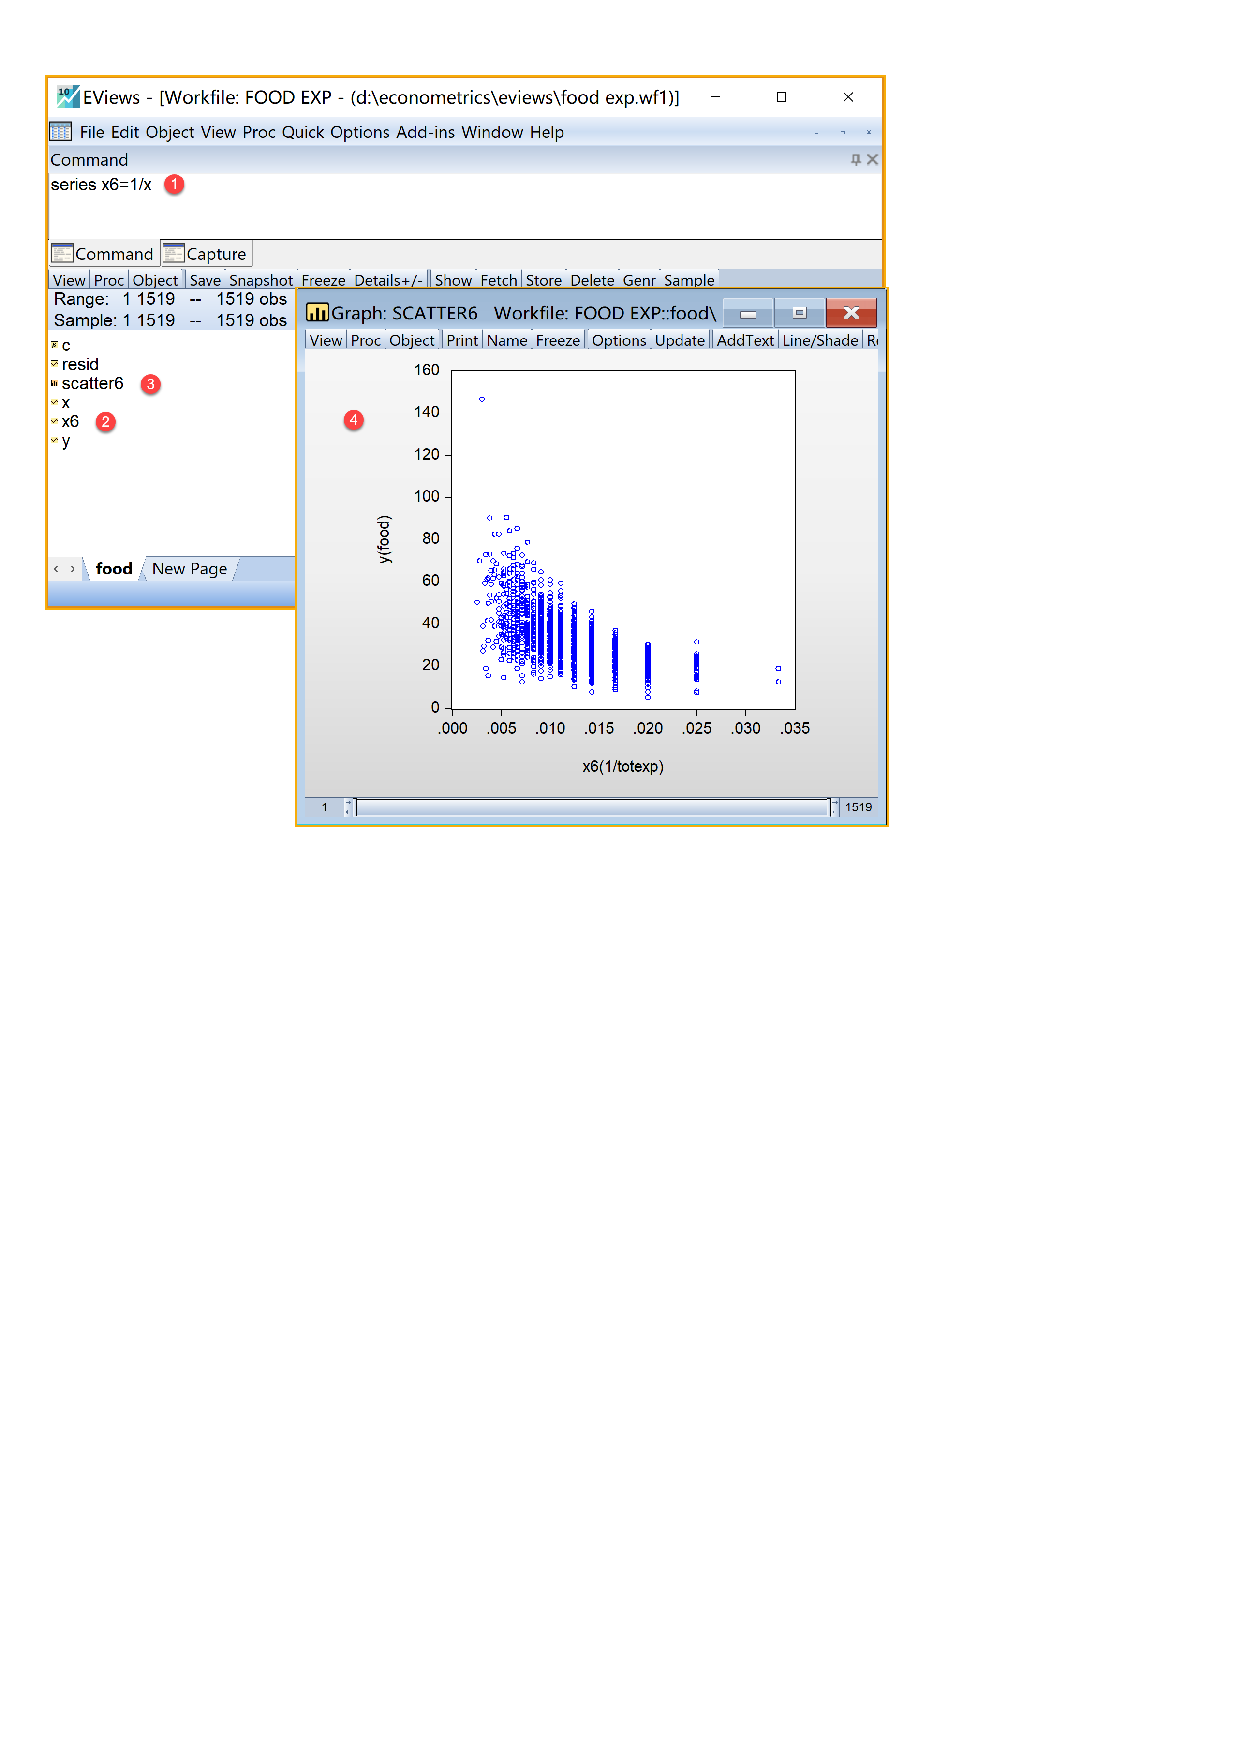
\includegraphics[width=24.22in,height=8in]{picture/lab3-model-function/scatter6} 

}

\caption{变换数据并绘制散点图}\label{fig:scatter}
\end{figure}

\hypertarget{m_6eviews}{%
\subsection{\texorpdfstring{对倒数模型\(M_6\)进行Eviews回归分析并提取回归系数}{对倒数模型M\_6进行Eviews回归分析并提取回归系数}}\label{m_6eviews}}

\begin{itemize}
\item
  Eviews操作目标:得到\(Y_i\)相对于\(1/X_i\)的Eviews回归报告,提取回归系数
\item
  Eviews操作思路:

  \begin{itemize}
  \item
    利用常规流程获得Eviews回归分析:

    \begin{itemize}
    \tightlist
    \item
      菜单操作:Quick--\textgreater{}estimate equation--\textgreater{}
      \texttt{y\ c\ 1/x}
    \end{itemize}
  \item
    保存好分析报告(建议命名为m6):

    \begin{itemize}
    \tightlist
    \item
      菜单操作:Name--\textgreater{}m6
    \end{itemize}
  \item
    提取报告中的回归系数(建议命名为\texttt{coef6}):

    \begin{itemize}
    \tightlist
    \item
      命令操作:\texttt{coef\ coef6=c}
    \end{itemize}
  \end{itemize}
\item
  Eviews操提示:两个Eviews模型内置对象(
\includegraphics{picture/object/Beta.png}C和
\includegraphics{picture/object/Series.png}rsid)

  \begin{itemize}
  \item
    
\includegraphics{picture/object/Beta.png}C和
\includegraphics{picture/object/Series.png}rsid都是Eviews模型内置对象,一旦建立workfile就会系统产生,用户不能对它进行删除或重命名(delete
    or rename)操作。

    \begin{itemize}
    \tightlist
    \item
      
\includegraphics{picture/object/Beta.png}C属于\textbf{系数}对象(\href{http://www.eviews.com/help/helpintro.html\#page/content\%2Fcoefcmd-coef_2.html\%23ww184054}{coef
      object}),这类对象主要用于表示系数列向量(coefficient column
      vector)。
\includegraphics{picture/object/Beta.png}C是用来装载回归模型的系数\(\hat{\beta}_1\)和\(\hat{\beta}_2\)\ldots{}\ldots{}
    \item
      \includegraphics{picture/object/series.png}resid属于\textbf{序列}对象(\href{http://www.eviews.com/help/helpintro.html\#page/content\%2Fseriescmd-series_2.html\%23ww203659}{series
      object}),这类对象主要用于表示序列(series)。\includegraphics{picture/object/series.png}resid是用来装载回归模型的残差\(e_i\)
    \end{itemize}
  \item
    
\includegraphics{picture/object/Beta.png}C和
\includegraphics{picture/object/Series.png}rsid是``临时容器''。它们只会装载最近一次Eviews建模分析(Estimate
    Equation)时的回归系数\(\hat{\beta}_i\)和回归残差\(e_i\)。一旦用户进行了新的Eviews建模分析(Estimate
    Equation)操作,它们就立即会被最新回归建模的系数和残差信息所``更新''。
  \item
    如果用户要创建多个回归方程,又想保留每个回归方程的回归系数\(\hat{\beta}_i\)和残差\(e_i\),可以通过下面两种方法将结果从``临时容器''中提取出来,并保存到指定的对象中去:

    \begin{itemize}
    \tightlist
    \item
      键鼠操作法。对
\includegraphics{picture/object/Beta.png}C或
\includegraphics{picture/object/Series.png}rsid右键拷贝(copy),然后在窗口区粘贴(paste),并进行重命名,保存。
    \item
      命令操作法。 *
      在命令窗口中输入Eviews命令\texttt{coef\ c01=c},即可得到当前回归模型系数
\includegraphics{picture/object/Beta.png}C的复制品\texttt{c01}(用户可以自己定义对象名称)。
      *
      在命令窗口中输入Eviews命令\texttt{series\ resid01=resid},即可得到当前回归模型系数\includegraphics{picture/object/series.png}resid的复制品\texttt{resid01}(用户可以自己定义对象名称)。
    \end{itemize}
  \item
    ``临时容器''
\includegraphics{picture/object/Beta.png}C和
\includegraphics{picture/object/Series.png}rsid按照Eviews建模先后次序不断被``更新''信息(分别是回归系数和残差序列)。``更新''基本原则是``依次占据对象的空间位置''。

    \begin{itemize}
    \tightlist
    \item
      回归方程的系数\(\hat{\beta}_i\)会依次占据
\includegraphics{picture/object/Beta.png}C对象的第1个单元格、第2个单元格、\ldots{}\ldots{},回归系数个数占据空间位置的多少因模型方程的不同而不同。尤其要注意的情形是:上一次操作回归模型的回归系数多,而最近一次操作回归模型的回归系数少。
    \item
      回归方程的残差\includegraphics{picture/object/series.png}resid在同一个工作文件(workfile)下,用户进行各类模型操作的样本数大多保持相同,因此,最近依次模型操作一般都会``完全更新''上一次模型操作的残差序列。
    \end{itemize}
  \end{itemize}
\end{itemize}

\begin{figure}

{\centering 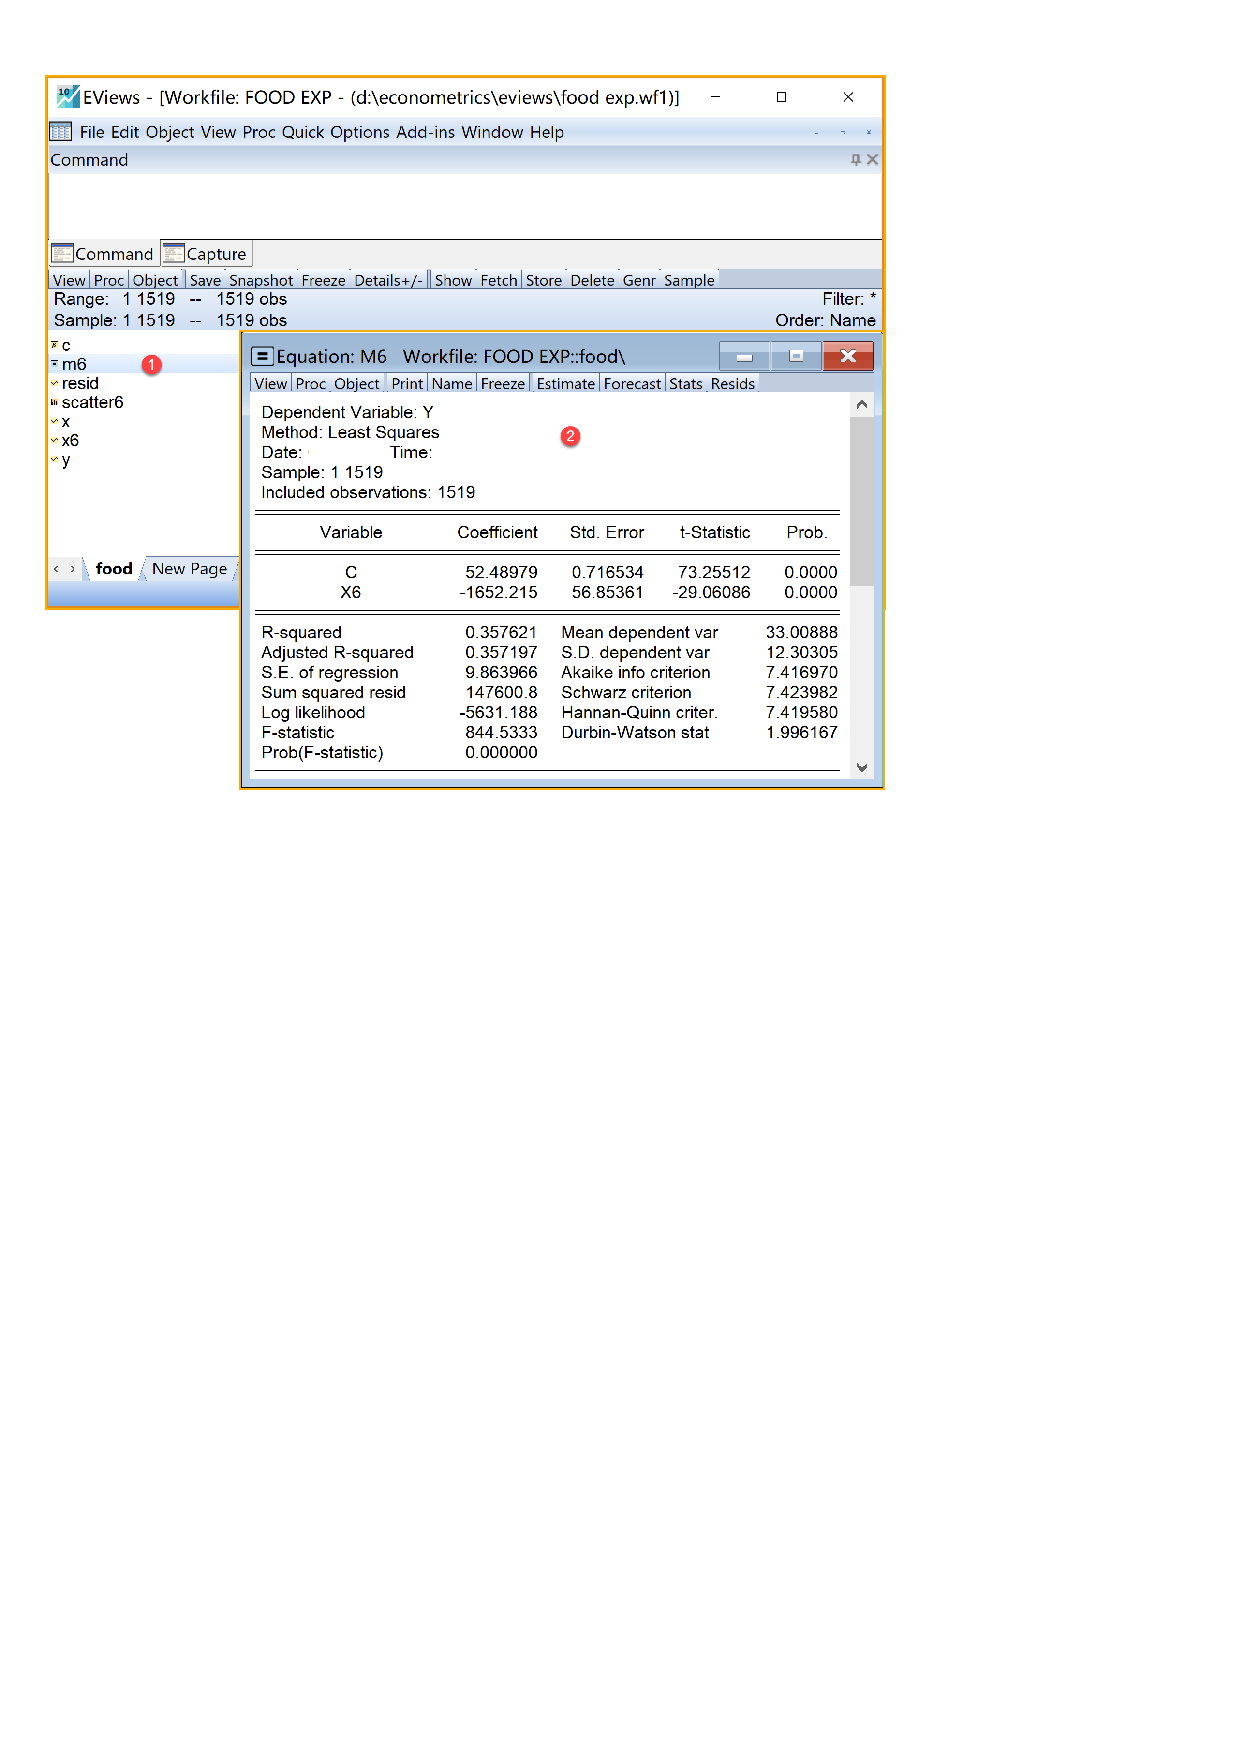
\includegraphics[width=24.14in,height=8in]{picture/lab3-model-function/equation6} 

}

\caption{构造倒数模型的回归方程}\label{fig:equation6}
\end{figure}

\begin{figure}

{\centering 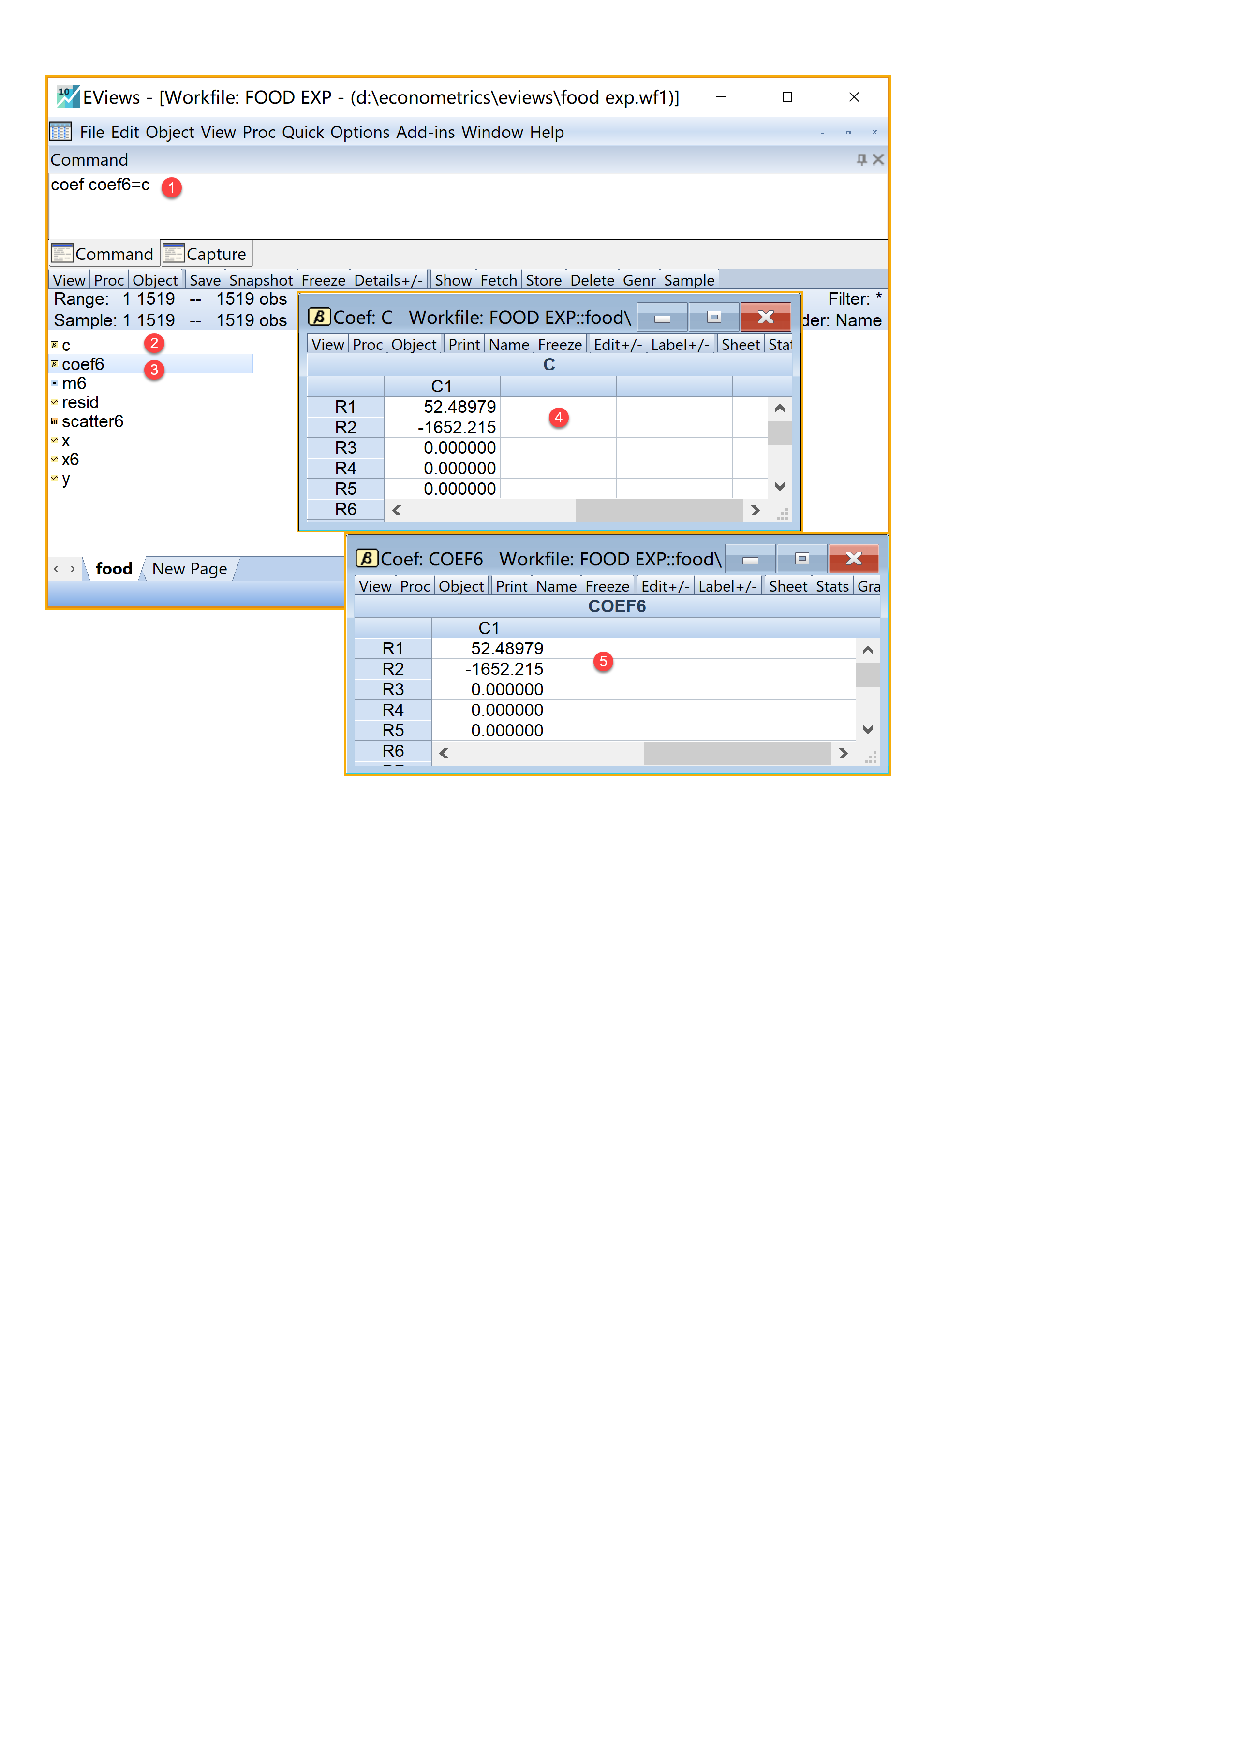
\includegraphics[width=24.31in,height=8in]{picture/lab3-model-function/coef6} 

}

\caption{提取回归方程的系数}\label{fig:coef6}
\end{figure}

\hypertarget{m_6yxx_0100y_030slope}{%
\subsection{\texorpdfstring{倒数模型\(M_6\)情形下,计算Y相对于X的点斜率\((X_0=100,Y_0=30)\)点斜率(slope)}{倒数模型M\_6情形下,计算Y相对于X的点斜率(X\_0=100,Y\_0=30)点斜率(slope)}}\label{m_6yxx_0100y_030slope}}

\begin{itemize}
\item
  Eviews操作目标:得到Y相对于X的点斜率\((X_0=100,Y_0=30)\)点斜率(slope)

  \begin{itemize}
  \item
    总体回归模型(PRM):\(Y_i=\beta_1+\beta_2/X_i+u_i\)
  \item
    点斜率计算公式:\(\beta_2/X_i^2\)
  \end{itemize}
\item
  Eviews操作思路:

  \begin{itemize}
  \item
    提取\texttt{coef6}的第二个值(也即\(\hat{\beta}_2\)),利用斜率公式计算得到Y相对于X的点斜率(建议命名为slp6):

    \begin{itemize}
    \tightlist
    \item
      命令操作:\texttt{scalar\ slp6=\ -coef6(2)/100\^{}2}
    \end{itemize}
  \end{itemize}
\end{itemize}

\begin{figure}

{\centering 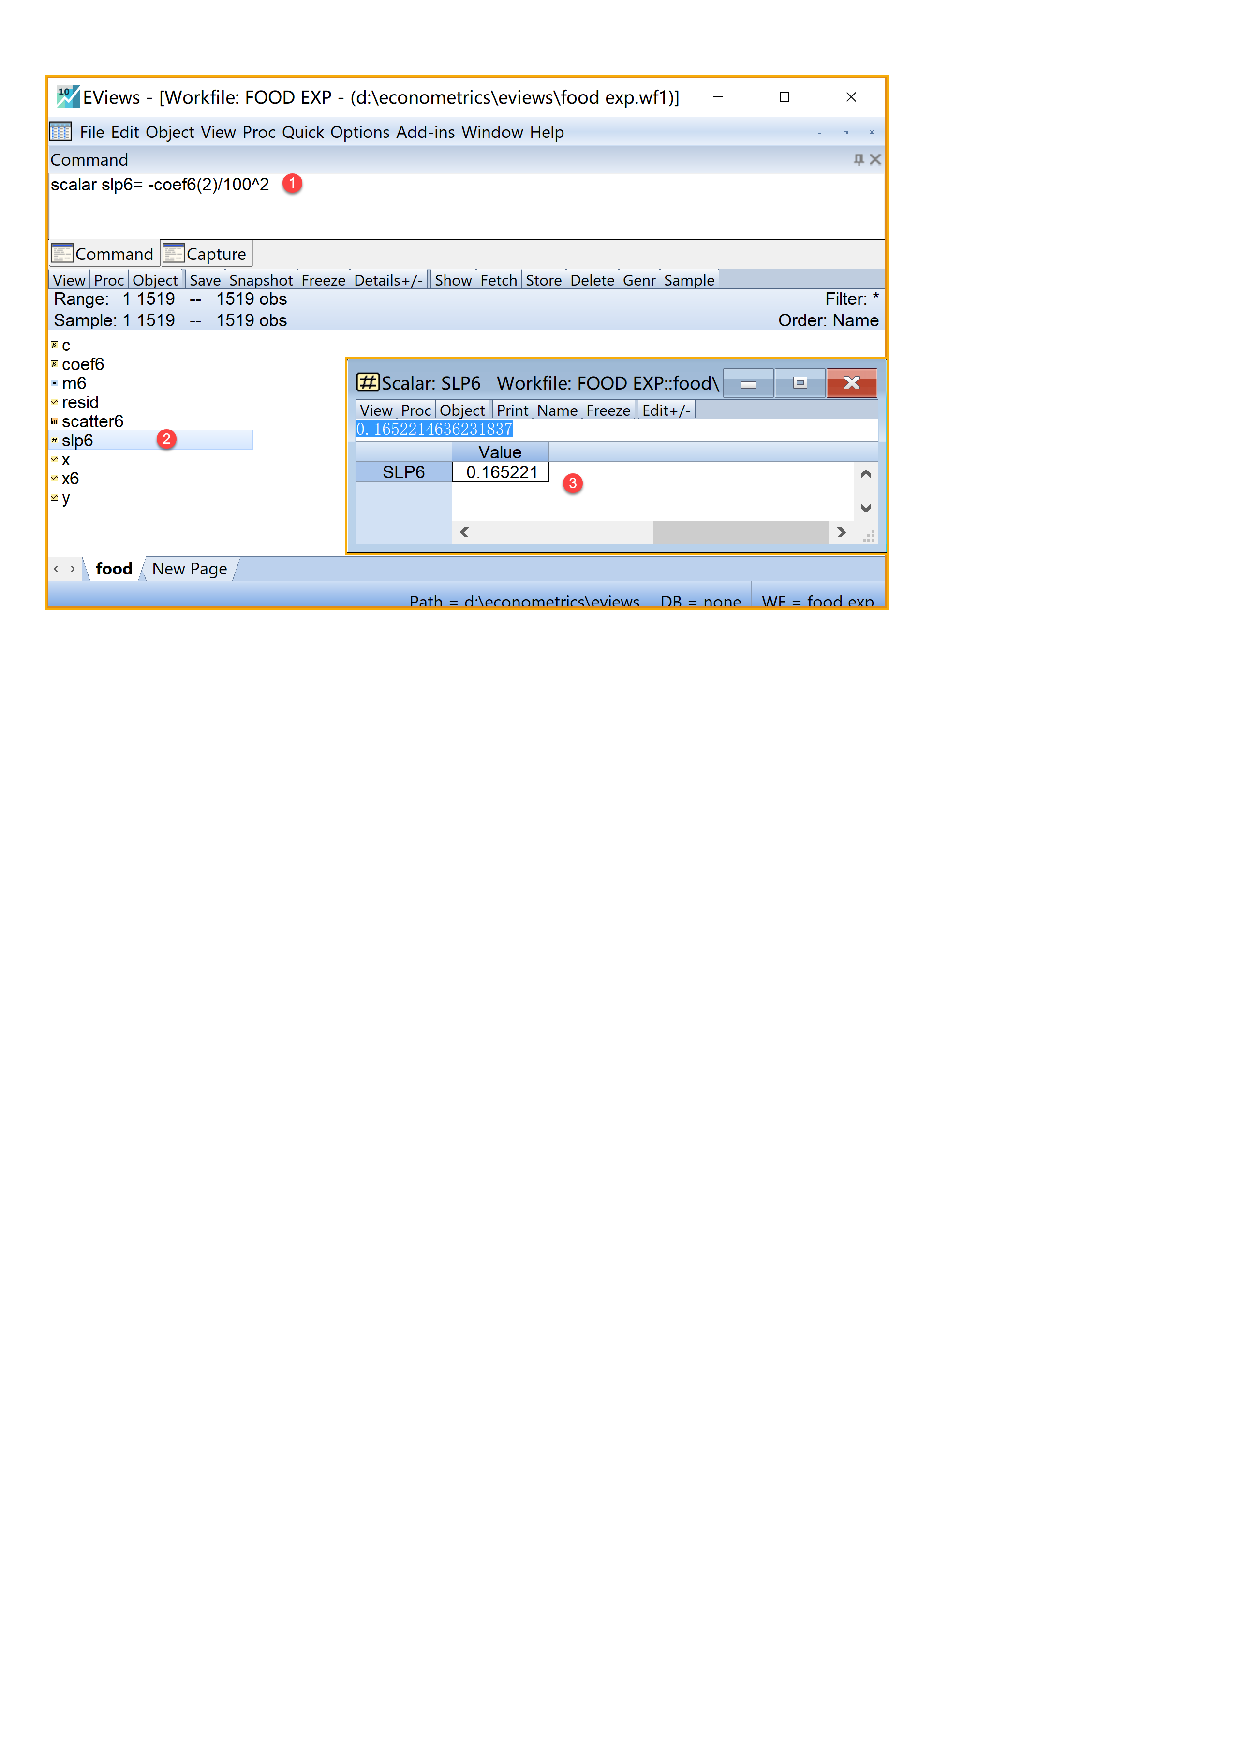
\includegraphics[width=24.24in,height=8in]{picture/lab3-model-function/slope6} 

}

\caption{得到Y对X的点斜率}\label{fig:slope6}
\end{figure}

\hypertarget{m_6yxelasticity}{%
\subsection{\texorpdfstring{倒数模型\(M_6\)情形下,计算Y相对于X的平均弹性(elasticity)}{倒数模型M\_6情形下,计算Y相对于X的平均弹性(elasticity)}}\label{m_6yxelasticity}}

\begin{itemize}
\item
  Eviews操作目标:得到Y相对于X的平均弹性(elasticity)

  \begin{itemize}
  \item
    总体回归模型(PRM):\(Y_i=\beta_1+\beta_2/X_i+u_i\)
  \item
    平均弹性计算公式:\(-\beta_2/(\bar{X}\bar{Y}\)
  \end{itemize}
\item
  Eviews操作思路:

  \begin{itemize}
  \item
    求出标量\(\bar{X}\)和\(\bar{Y}\)(建议分别命名为x\_mean和y\_mean):

    \begin{itemize}
    \item
      命令操作:\texttt{scalar\ x\_mean=@mean(x)}
    \item
      命令操作:\texttt{scalar\ y\_mean=@mean(y)}
    \end{itemize}
  \item
    提取\texttt{coef6}的第二个值(也即\(\hat{\beta}_2\)),利用平均弹性公式计算得到Y相对于X的平均弹性(建议命名为els6):

    \begin{itemize}
    \tightlist
    \item
      命令操作:\texttt{scalar\ els6=\ -coef6(2)/(x\_mean*y\_mean)}
    \end{itemize}
  \end{itemize}
\end{itemize}

\begin{figure}

{\centering 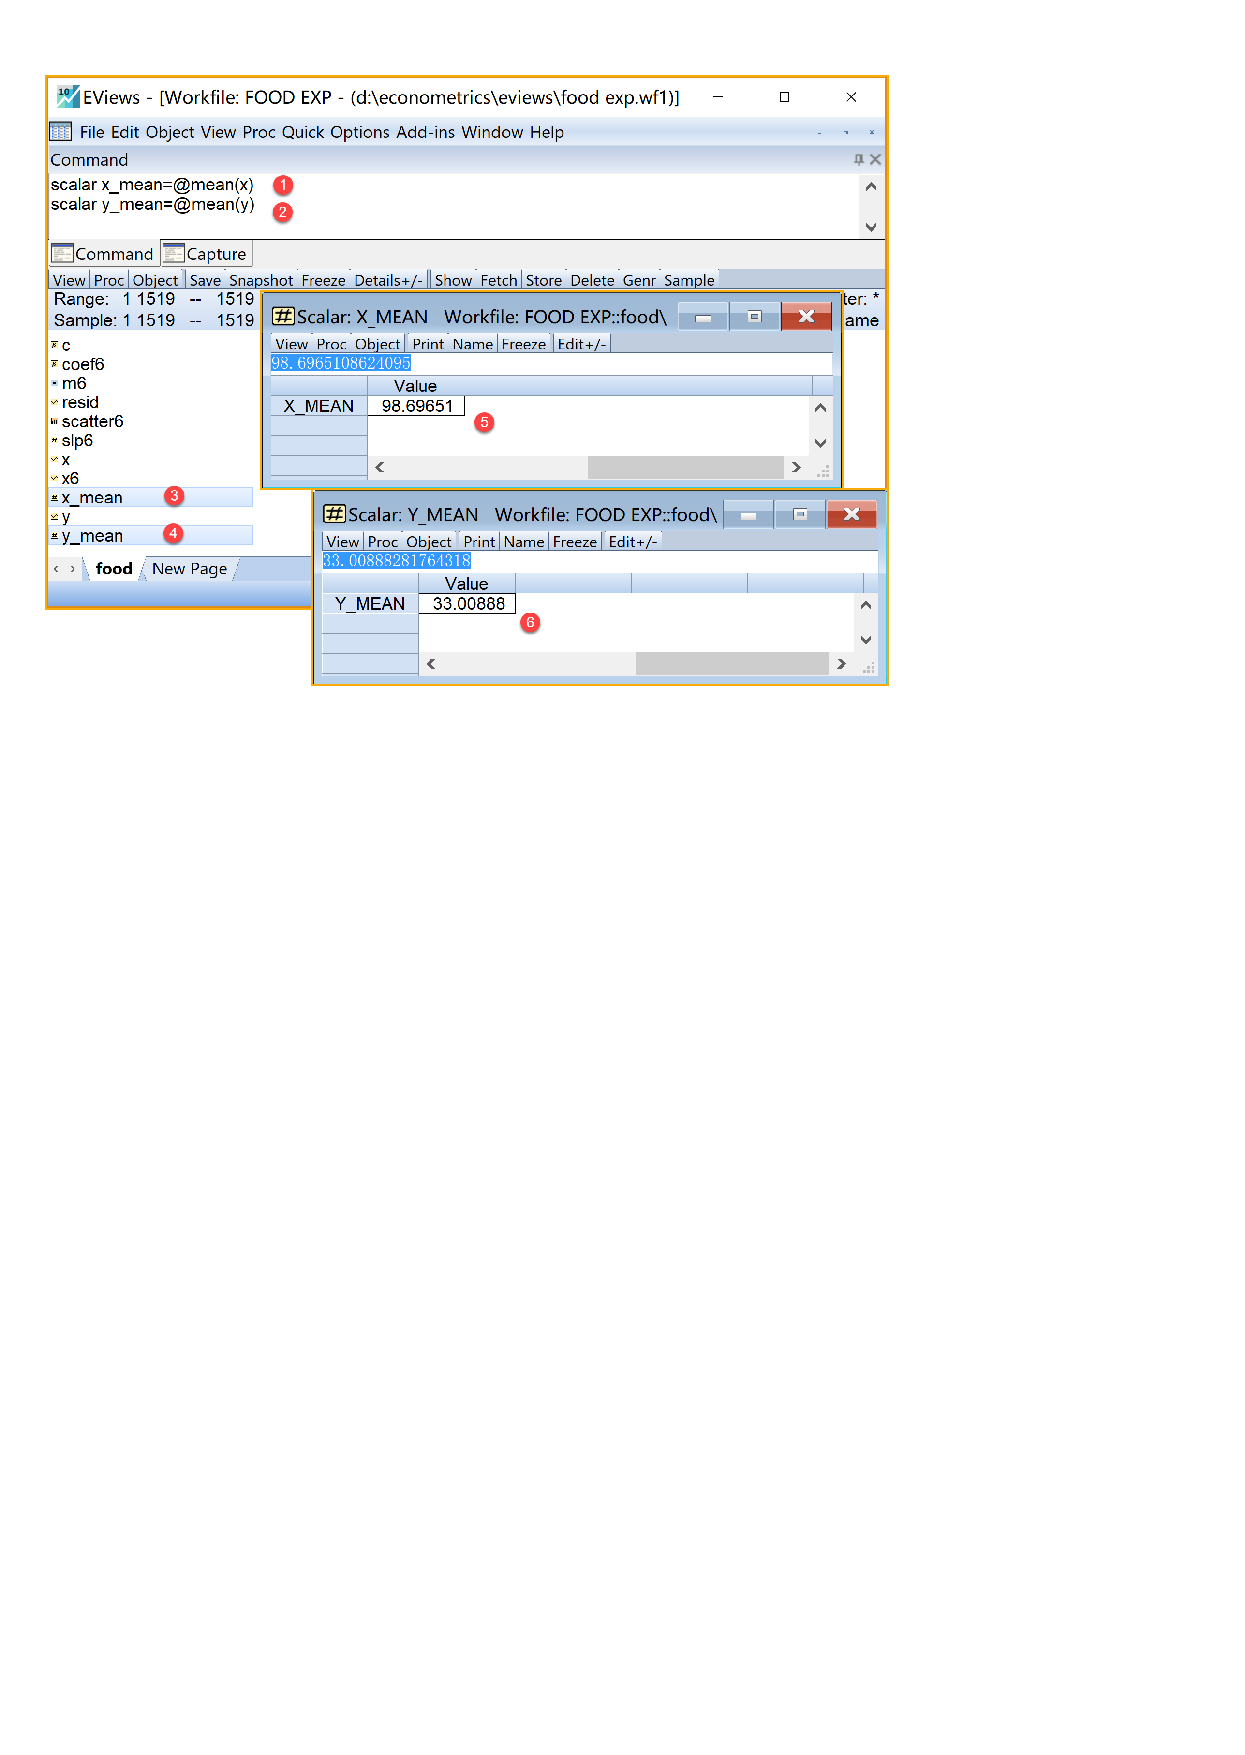
\includegraphics[width=24.24in,height=8in]{picture/lab3-model-function/mean6} 

}

\caption{得到Y和X的均值}\label{fig:mean6}
\end{figure}

\begin{figure}

{\centering 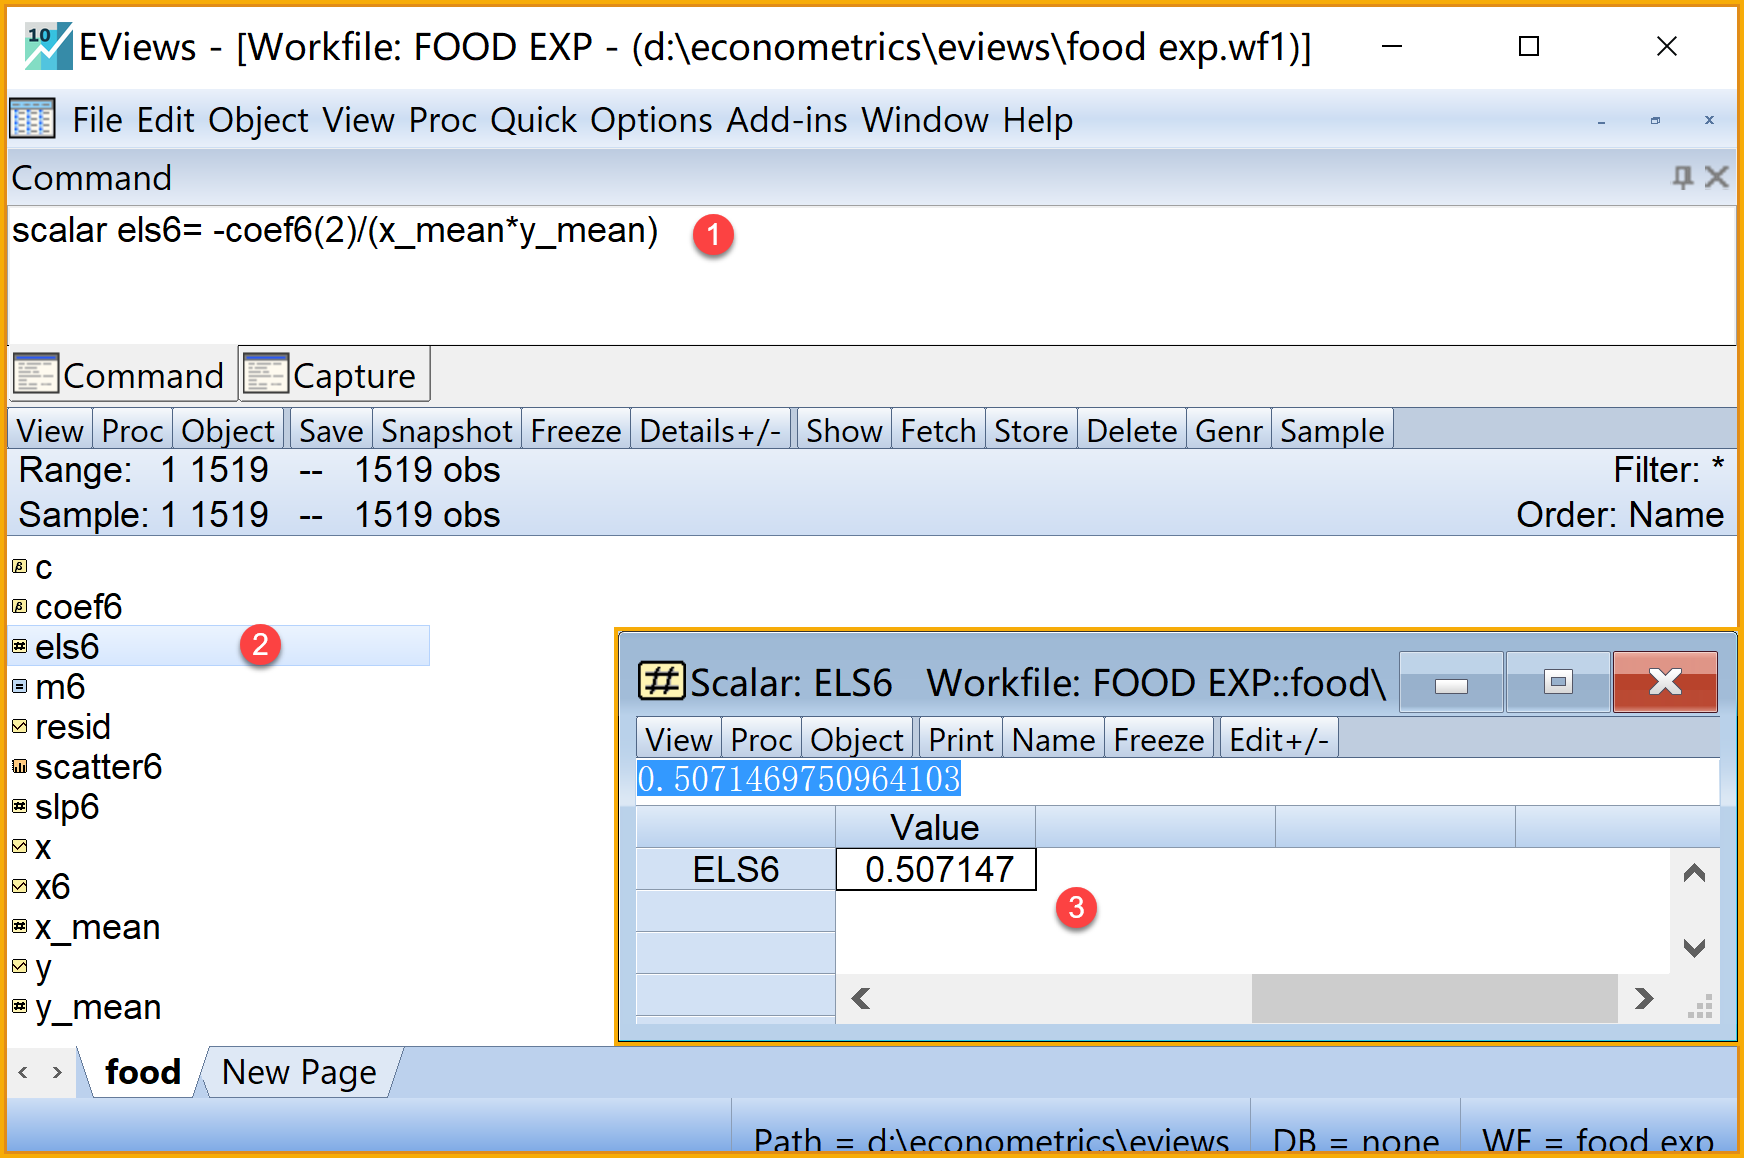
\includegraphics[width=24.22in,height=8in]{picture/lab3-model-function/elasticity6} 

}

\caption{得到Y对X的平均弹性}\label{fig:elasticity6}
\end{figure}


\end{document}
